\subsection{Analysis of the Frequency Spectra of Different Drums and Cymbals} 
\label{section:classificationSpectrumAnalysis}

Before a classification algorithm can be applied to a drum sound frame, it needs to be searched for significant features. To find those features, the time and frequency domains of each used drum and cymbal are examined. The aim of this analysis is to find features that enable to distinguish between the components of the used drum set. There were recorded different stroke types on every component.  The recordings were made with a sampling rate of 44.1 kHz and a resolution of 16 bit. The frequency spectrum of the drum strokes is calculated by finding the onset and applying MatLab\textsuperscript{\textregistered}s built in FFT algorithm with a window size of 2048 and a hamming window.

First, the different drums are considered. These are a bass drum, snare drum, two rack toms (tom 1, tom 2) and one floor tom (tom 3). Subsequently, the cymbals are analyzed. Used cymbals are the hi-hat, which can be played opened or closed, a crash cymbal and a ride cymbal. For each drum or cymbal, different kinds of strokes are considered. Drums can be stroked on their center or at the edge and a cymbal at its rim, bow or bell. Moreover, a stroke can be performed with low or high power. Each kind of stroke can produce a slightly different sound and frequency spectrum.

It is observed that the main frequency bins of a drum sound are located in the frequency band from 40 Hz to 1000 Hz and those of a cymbal in a much broader frequency band from 40 Hz to 10.000 Hz or higher. Thus, in the following a frequency spectrum from 0 Hz to 1000 Hz for the drums and from 0 Hz to 10000 Hz for the cymbals is considered.

There are three different graphics created for each drum stroke. The first graphic shows the time domain with a marked window of 2048 samples, beginning at the onset of the stroke. Further on, it shows the frequency spectrum of the marked window either from 0 Hz to 1000 Hz or from 0 Hz to 10.000 Hz, depending on the occurrence of frequency peaks in the spectrum. The second graphic is created by MatLab\textsuperscript{\textregistered}s build in spectrogram function. It displays the frequency domain in the x-axis and the time domain in the y-axis. The frequency amplitudes are displayed by blue- and red-intensities of colored rectangles. The more red a color rectangle contains, the higher is the frequency amplitude at this point. Blue signals a low frequency amplitude. Thus, this graphic shows how the frequency spectrum of an entire stroke develops over time. The third graphic displays frequency spectra of three subsequent frames with a window size of 1024 and an overlap length of 512. Here, it can be analyzed how the frequency spectrum develops within first 2028 samples. This gives information about the steadiness of the examined sound.

%While a drum (except the snare drum) produces a few explicit frequency peaks, a cymbal produces lots of peaks with varying relations between amplitudes while a stroke and also between different drum strokes.


% Farblegende zu spectrogram hinzufügen!!!

\subsubsection{Bass Drum}

The bass drum is played with a felt covered mallet that is stroked against the drum head by the use of a foot pedal. Hence, the bass drum is always hit at the same point with similar power. So only one kind of stroke needs to be considered here

A stroke on the bass drum creates a very low frequent sound. The frequency spectrum shows two major frequency peaks at 86.1 Hz and 172.3 Hz and a smaller peak at 258.3 Hz \ref{fig:bass1}. The spectrogram in figure \ref{fig:bass2} shows that the peaks at 86.1 Hz and 258.3 Hz decay earlier than the peak at 172.3 Hz. 

\begin{figure}[hbp]
	\centering
	\subfloat[%
			\newline
			Top: Time Domain
			\newline
			Center: Frequency domain from 0 to 10 kHz
			\newline
			Bottom: Frequency domain from 0 to 1000 Hz
		]{
		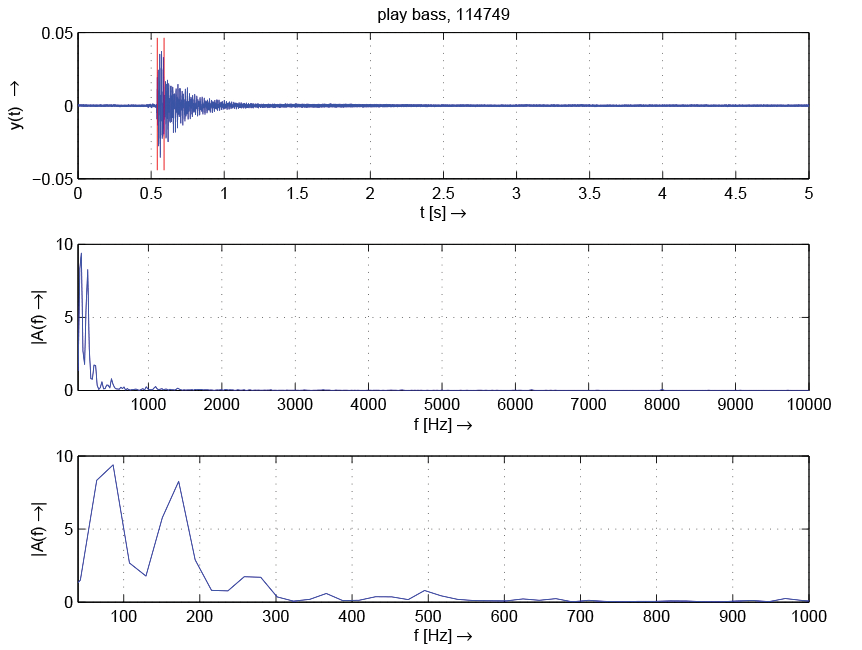
\includegraphics[width=7.3cm]{images/drum_spectra/play_bass_114749_2048_0_plot_01.png}
		\label{fig:bass1}
	}
	\qquad
	\subfloat[%
			\newline 
			Spectrogram of frequency peak intensities from 0 to 1000 Hz with fft-length of 2048 and an overlap length of 1024 displayed in time domain.
		]{
		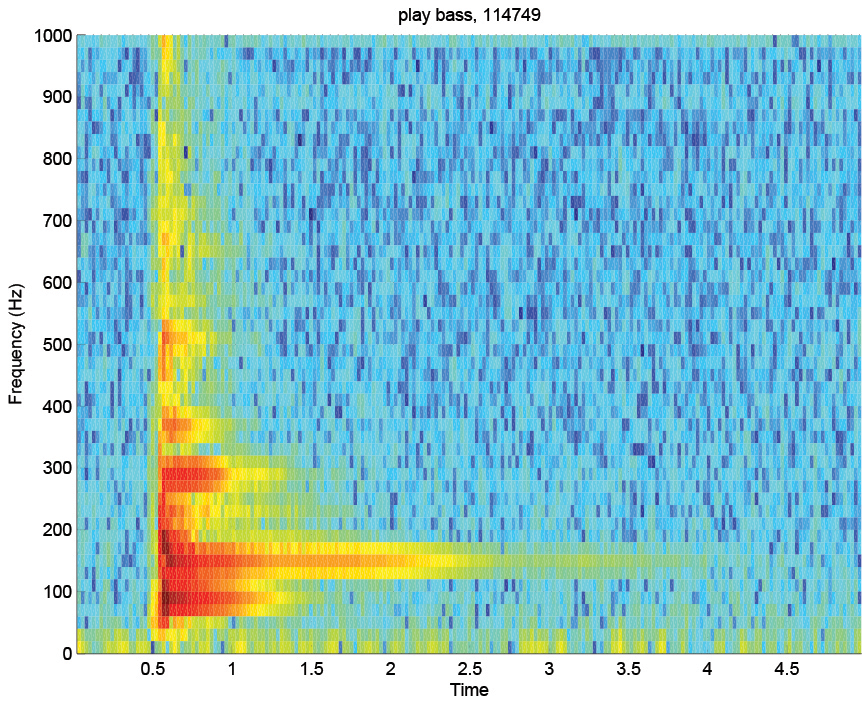
\includegraphics[width=7.3cm]{images/drum_spectra/play_bass_114749_2048_0_plot_03.png}
		\label{fig:bass2}
	}
	\caption{Stroke on a bass drum.}
	\label{fig:bass}
\end{figure}


\subsubsection{Tom Toms}

For the three tom toms, there are considered centered, non-centered, low and high powered strokes. For all strokes, there are explicit peaks in a frequency band from 40 Hz to 1000 Hz, which appear in all of the four stroke variants.
 
Figure \ref{fig:tom11} shows a centered stroke at tom 1. One outstanding peak is produced at 193.8 Hz and some smaller ones with higher frequency rates up to 1000 Hz. As shown in the spectrogram, there are peaks around 200 Hz, 300 Hz and 560 Hz persisting over time. The subsequent frames in figure \ref{fig:tom113} show that the peaks decrease but persist stable during the first 2048 samples. 

\begin{figure}
	\centering
	\subfloat[Time and frequency domain]{
		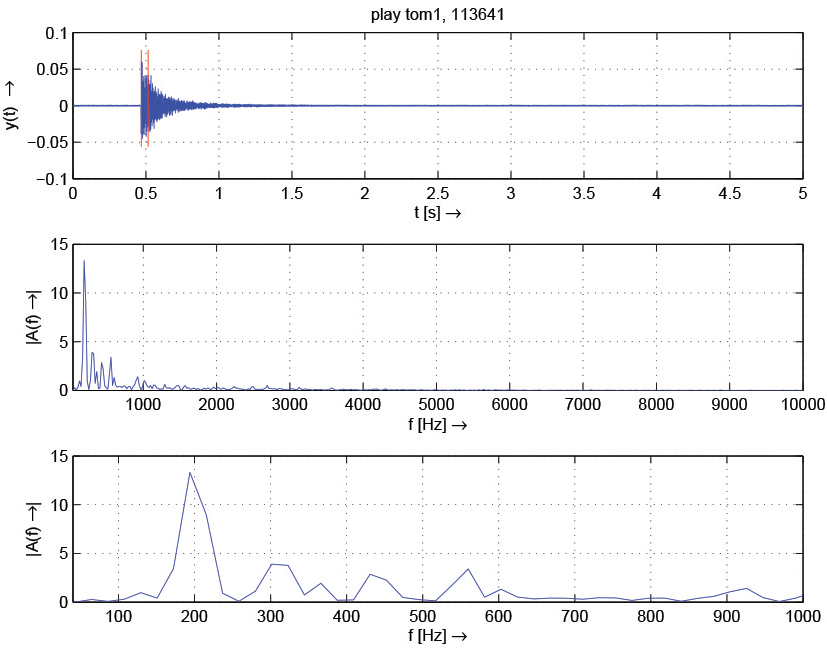
\includegraphics[height=5.5cm]{images/drum_spectra/play_tom1_113641_2048_0_plot_01_center.png}
		\label{fig:tom111}
	}
	\subfloat[Spectrogram]{
		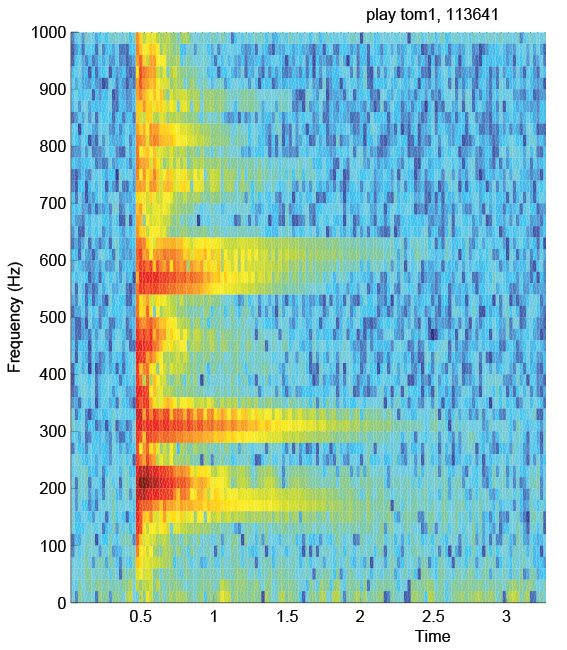
\includegraphics[height=5.5cm]{images/drum_spectra/play_tom1_113641_2048_0_plot_03_center.png}
		\label{fig:tom112}
	}
	\subfloat[Frames]{
		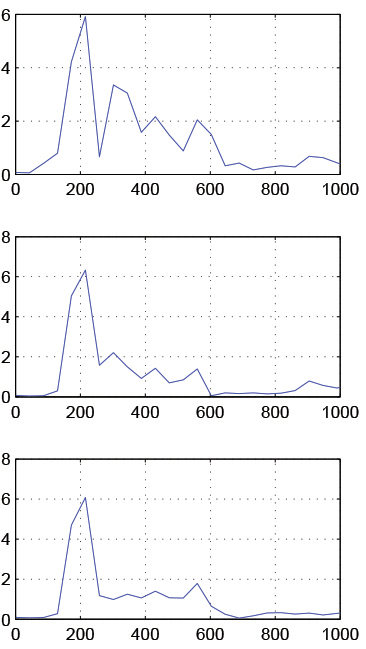
\includegraphics[height=5.5cm]{images/drum_spectra/play_tom1_113641_2048_0_plot_05_center.png}
		\label{fig:tom113}
	}
	\caption{Centered stroke on tom 1.}
	\label{fig:tom11}
\end{figure}

For a stroke at the edge of tom 1 the peaks remain the same, but the previously small peaks appears larger. The highest peak is still at 193.8 Hz. This can be seen in figure \ref{fig:tom12}.

\begin{figure}
	\centering
	\subfloat[Time and frequency domain]{
		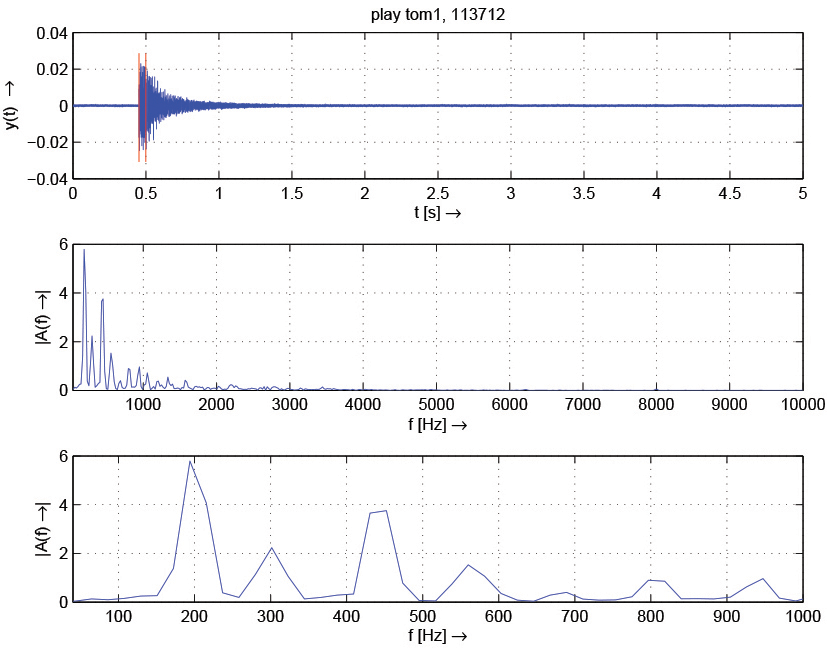
\includegraphics[height=5.5cm]{images/drum_spectra/play_tom1_113712_2048_0_plot_01_edge.png}
		\label{fig:tom121}
	}
	\subfloat[Spectrogram]{
		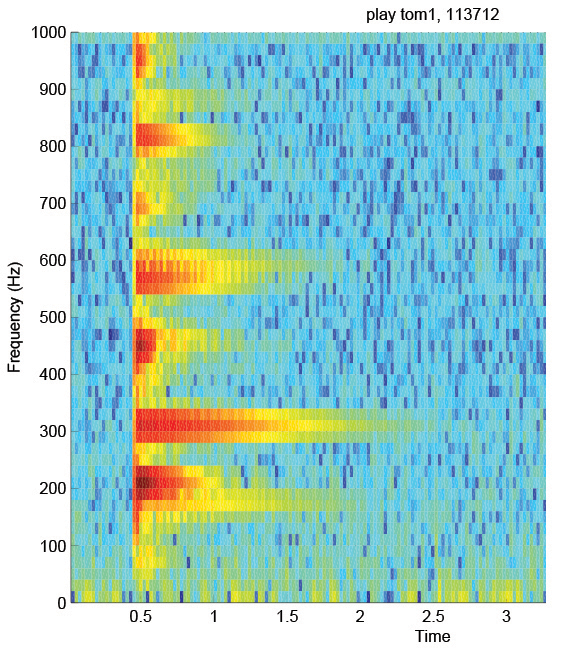
\includegraphics[height=5.5cm]{images/drum_spectra/play_tom1_113712_2048_0_plot_03_edge.png}
		\label{fig:tom122}
	}
	\subfloat[Frames]{
		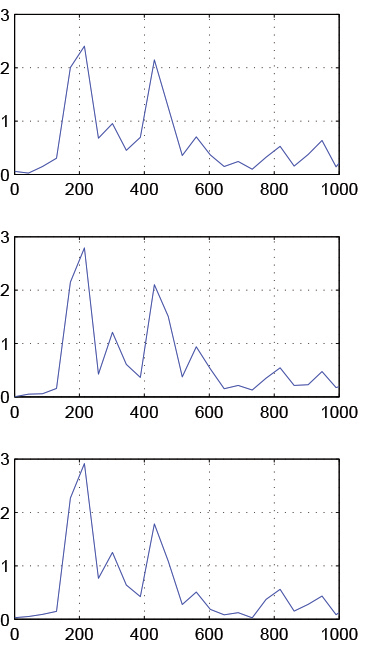
\includegraphics[height=5.5cm]{images/drum_spectra/play_tom1_113712_2048_0_plot_05_edge.png}
		\label{fig:tom123}
	}
	\caption{Stroke on the edge of tom 1.}
	\label{fig:tom12}
\end{figure}

Figure \ref{fig:tom13} shows a low powered and figure \ref{fig:tom14} a high powered centered stroke on tom 1. For the low powered stroke it is noticed that the peak at 193.8 Hz is not as significant as before anymore. Furthermore, if subsequent frames are considered, the frequency amplitudes are varying substantially in the first few milliseconds of the stroke. Later on, the sound stabilizes and only the known peaks persist (figure \ref{fig:tom132}). In contrast to the varying amplitudes of a low powered stroke, for a high powered one the peaks are explicit and remain stable over time. Thus, it can be expected that the higher the power of the stroke, the clearer the outstanding peak is separated from the others.

\begin{figure}
	\centering
	\subfloat[Time and frequency domain]{
		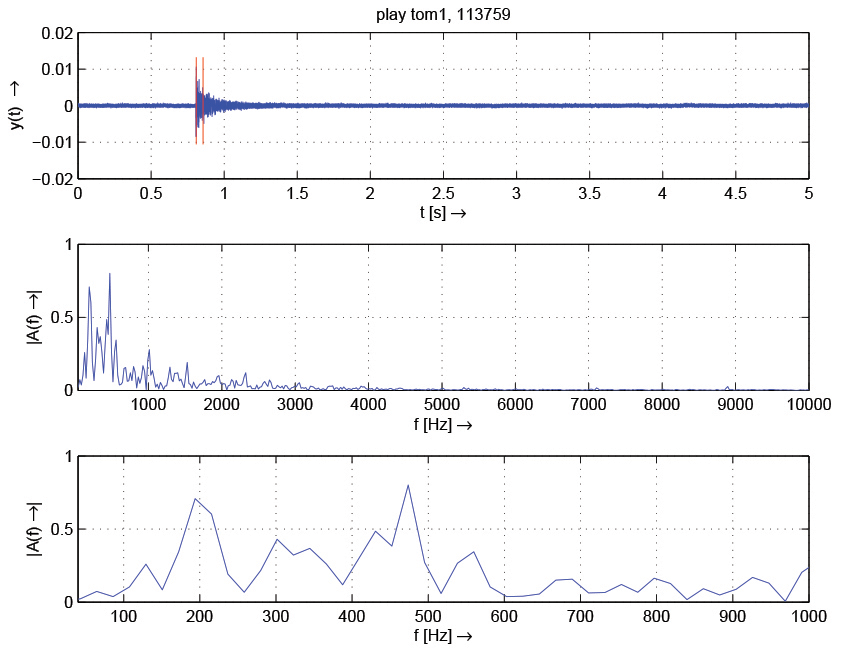
\includegraphics[height=5.5cm]{images/drum_spectra/play_tom1_113759_2048_0_plot_01_low.png}
		\label{fig:tom131}
	}
	\subfloat[Spectrogram]{
		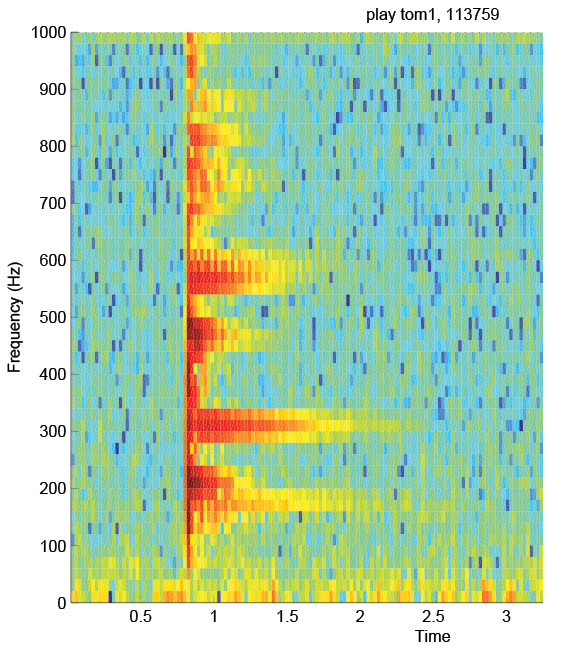
\includegraphics[height=5.5cm]{images/drum_spectra/play_tom1_113759_2048_0_plot_03_low.png}
		\label{fig:tom132}
	}
	\subfloat[Frames]{
		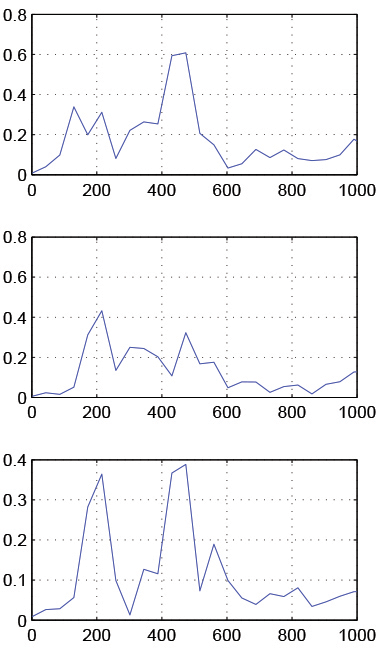
\includegraphics[height=5.5cm]{images/drum_spectra/play_tom1_113759_2048_0_plot_05_low.png}
		\label{fig:tom133}
	}
	\caption{Low powered centered stroke on tom 1.}
	\label{fig:tom13}
\end{figure}

\begin{figure}
	\centering
	\subfloat[Time and frequency domain]{
		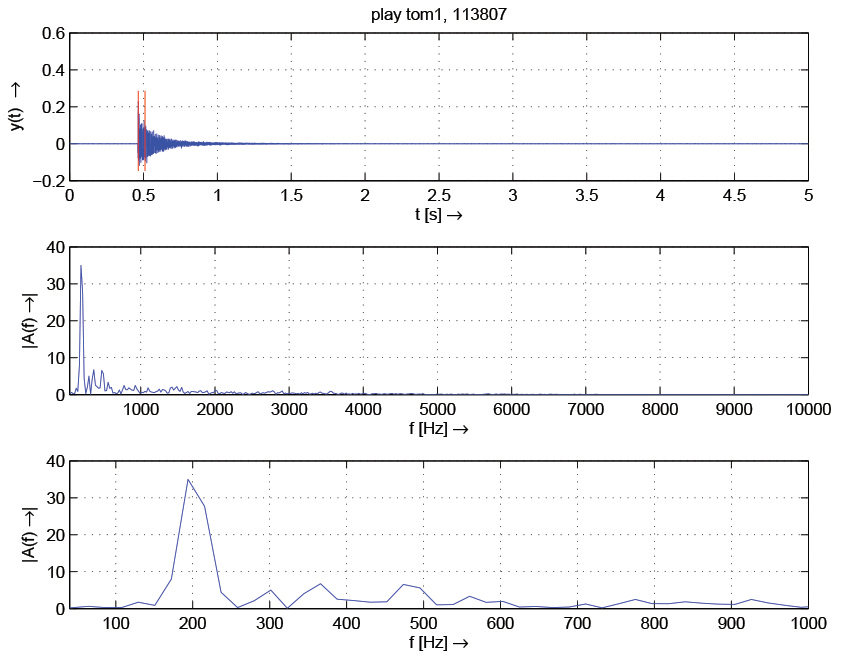
\includegraphics[height=5.5cm]{images/drum_spectra/play_tom1_113807_2048_0_plot_01_high.png}
		\label{fig:tom141}
	}
	\subfloat[Spectrogram]{
		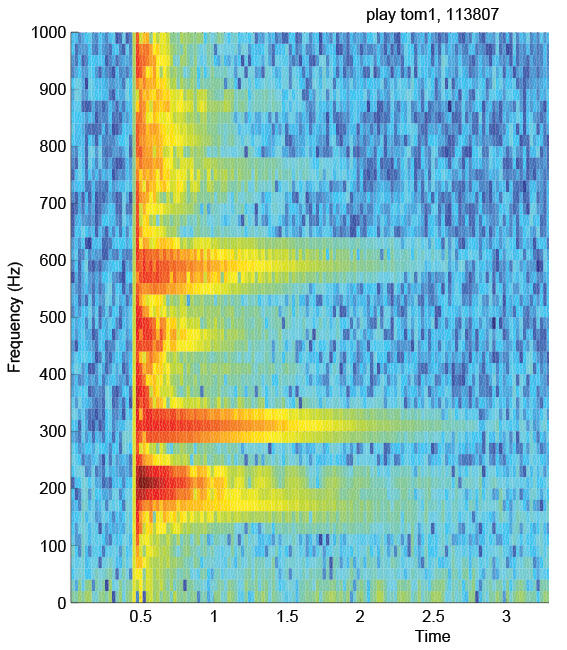
\includegraphics[height=5.5cm]{images/drum_spectra/play_tom1_113807_2048_0_plot_03_high.png}
		\label{fig:tom142}
	}
	\subfloat[Frames]{
		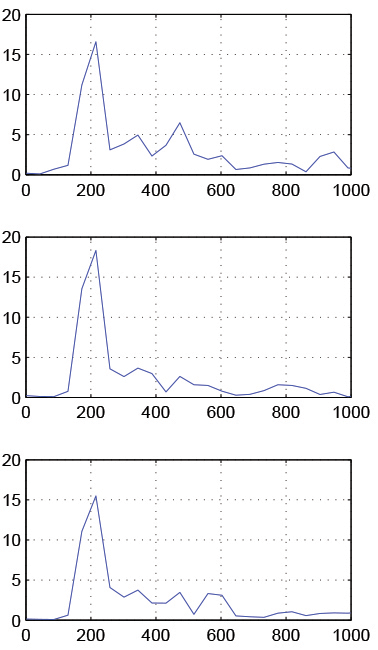
\includegraphics[height=5.5cm]{images/drum_spectra/play_tom1_113807_2048_0_plot_05_high.png}
		\label{fig:tom143}
	}
	\caption{High powered centered stroke on tom 1.}
	\label{fig:tom14}
\end{figure}


Tom 2 produces a lower sound than tom 1. It shows one single explicit peak at 172.3 Hz, which remains stable over time (figures \ref{fig:tom21}, \ref{fig:tom22} and \ref{fig:tom23}). It also is recognized that the lower frequency peaks are quite unstable and decay fast in contrast to the outstanding one. These smaller peaks appear higher and persist over time if the edge of tom 2 is stroked. Though, the peak at 172.3 Hz remains the highest one (figure \ref{fig:tom22}). This peak persists in both low and high powered strokes. 

\begin{figure}
	\centering
	\subfloat[Time and Frequency domain]{
		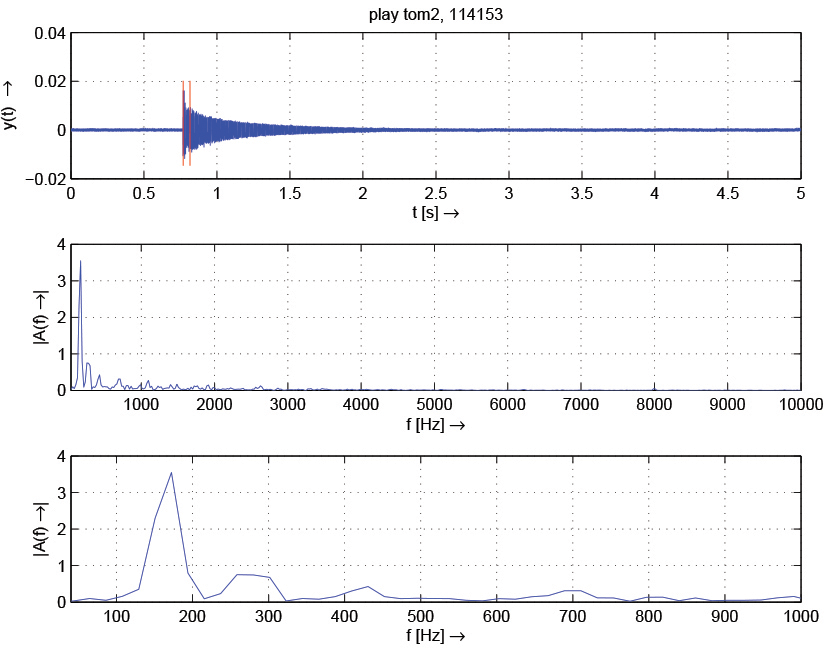
\includegraphics[height=5.5cm]{images/drum_spectra/play_tom2_114153_2048_0_plot_01_low.png}
		\label{fig:tom211}
	}
	\subfloat[Spectrogram]{
		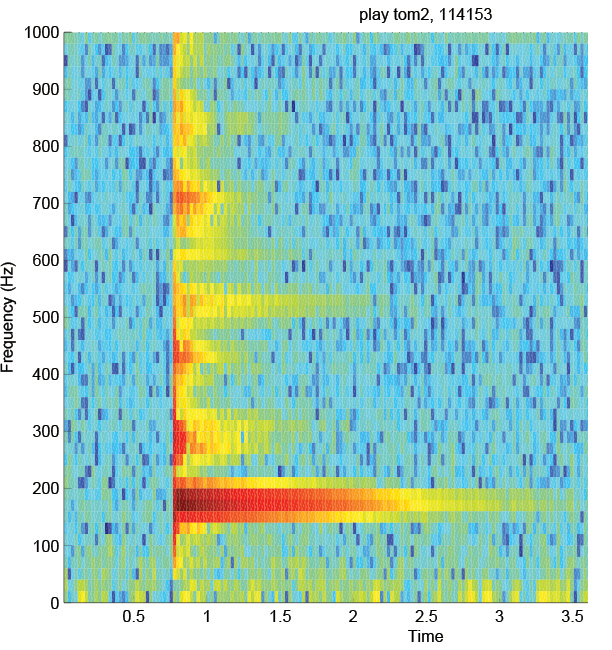
\includegraphics[height=5.5cm]{images/drum_spectra/play_tom2_114153_2048_0_plot_03_low.png}
		\label{fig:tom212}
	}
	\subfloat[Frames]{
		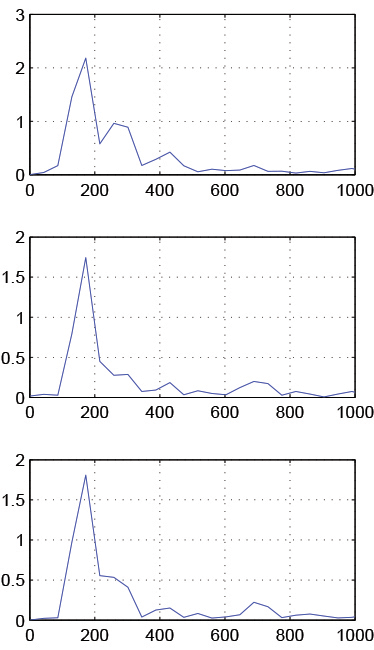
\includegraphics[height=5.5cm]{images/drum_spectra/play_tom2_114153_2048_0_plot_05_low.png}
		\label{fig:tom213}
	}
	\caption{Centered stroke with low power on tom 2.}
	\label{fig:tom21}
\end{figure}


\begin{figure}
	\centering
	\subfloat[Time and Frequency domain]{
		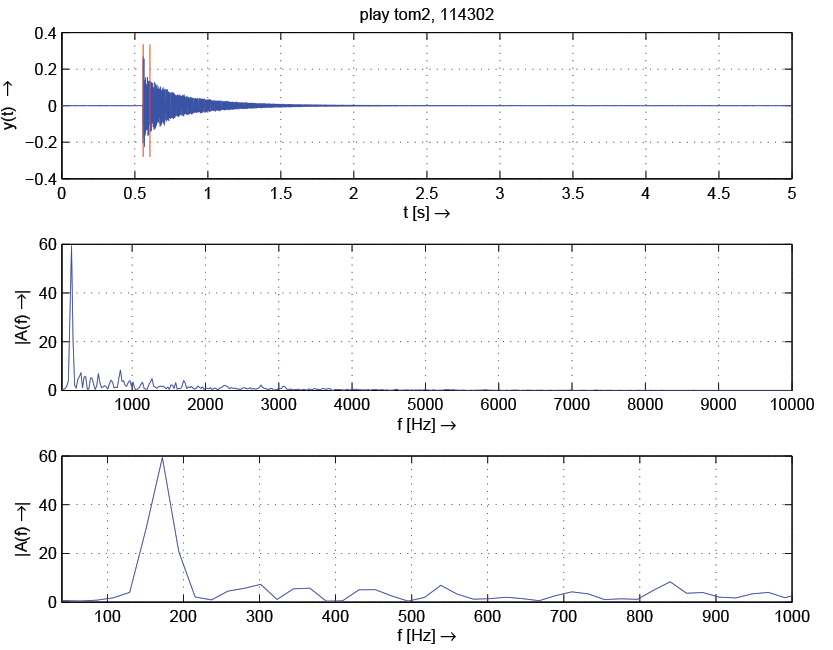
\includegraphics[height=5.5cm]{images/drum_spectra/play_tom2_114302_2048_0_plot_01_high.png}
		\label{fig:tom221}
	}
	\subfloat[Spectrogram]{
		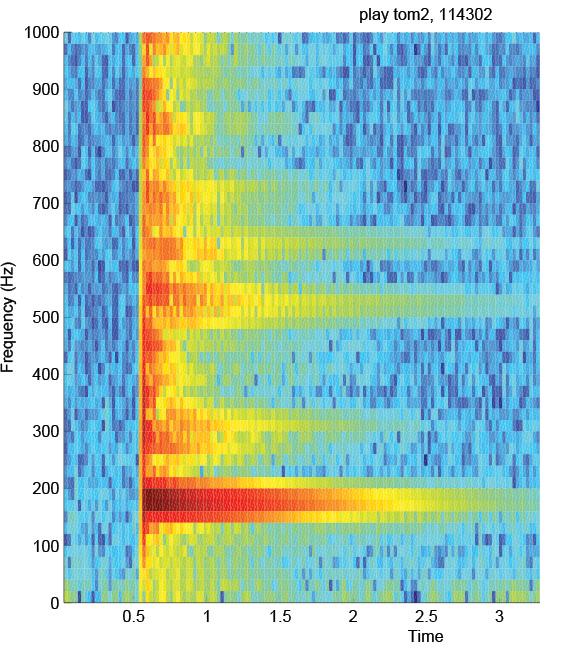
\includegraphics[height=5.5cm]{images/drum_spectra/play_tom2_114302_2048_0_plot_03_high.png}
		\label{fig:tom222}
	}
	\subfloat[Frames]{
		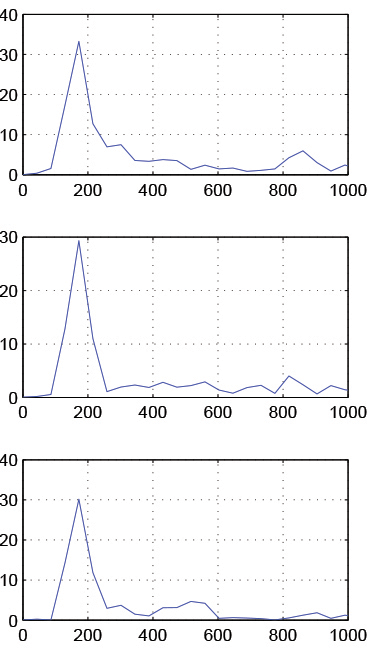
\includegraphics[height=5.5cm]{images/drum_spectra/play_tom2_114302_2048_0_plot_05_high.png}
		\label{fig:tom223}
	}
	\caption{Centered stroke with high power on tom 2.}
	\label{fig:tom22}
\end{figure}

\begin{figure}
	\centering
	\subfloat[Time and Frequency domain]{
		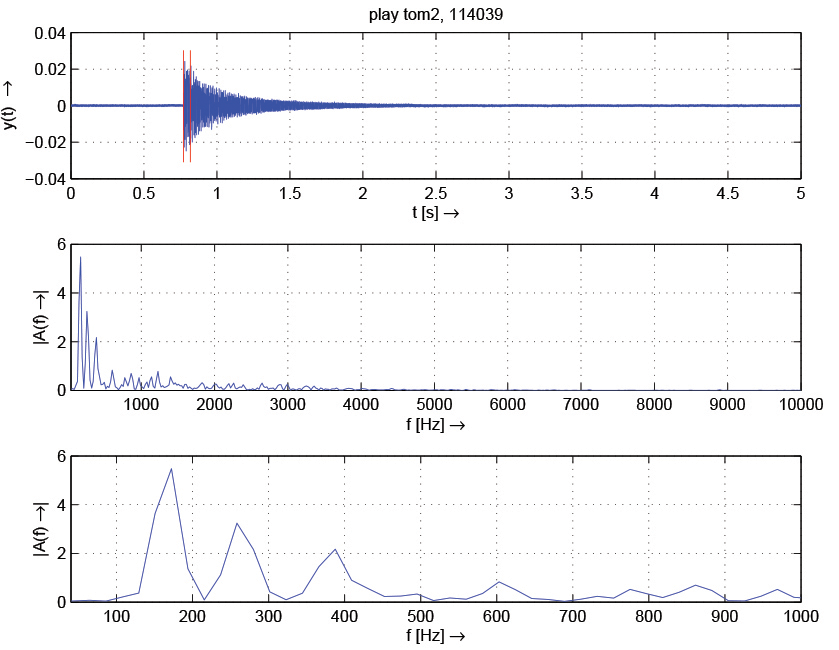
\includegraphics[height=5.5cm]{images/drum_spectra/play_tom2_114039_2048_0_plot_01_edge.png}
		\label{fig:tom231}
	}
	\subfloat[Spectrogram]{
		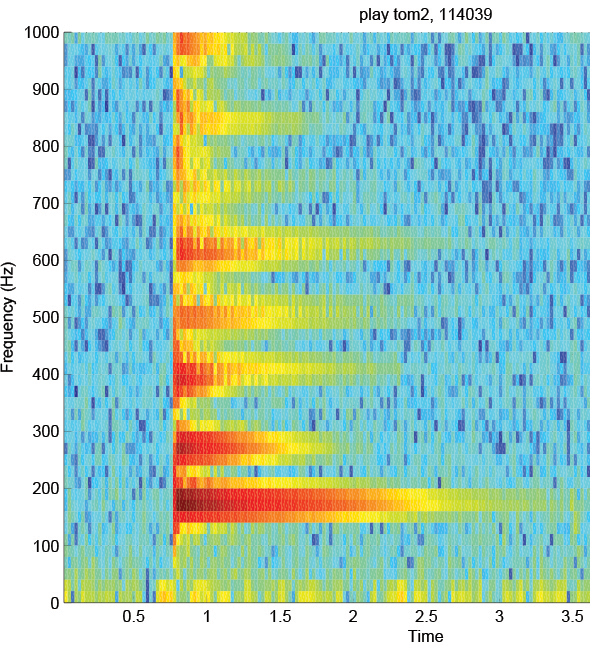
\includegraphics[height=5.5cm]{images/drum_spectra/play_tom2_114039_2048_0_plot_03_edge.png}
		\label{fig:tom232}
	}
	\subfloat[Frames]{
		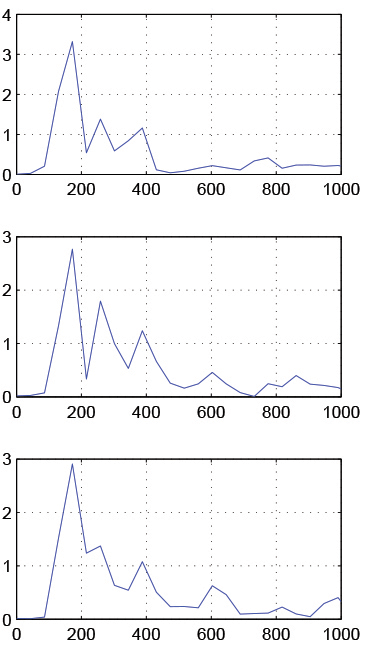
\includegraphics[height=5.5cm]{images/drum_spectra/play_tom2_114039_2048_0_plot_05_edge.png}
		\label{fig:tom233}
	}
	\caption{Stroke on the edge of tom 2.}
	\label{fig:tom23}
\end{figure}


Tom 3 produces the lowest frequent sound of all tested tom toms. It shows several outstanding peaks. The three highest ones appear at 172.3 Hz, 258.4 Hz and 387.6 Hz. 

If figures \ref{fig:tom31}, \ref{fig:tom32} and \ref{fig:tom33} are compared, it is recognized that the spectral shape changes its form, depending on if the stroke is low powered, high powered, centered or placed at the edge. The maximum peak appears shifted at 108.1 Hz for high powered strokes and 151.3 Hz for strokes at the edge. Just like tom 1 and tom 2, tom 3 shows its main peak clearer separated from the others if the stroke has more power. 

%TOM3
\begin{figure}
	\centering
	\subfloat[Time and Frequency domain]{
		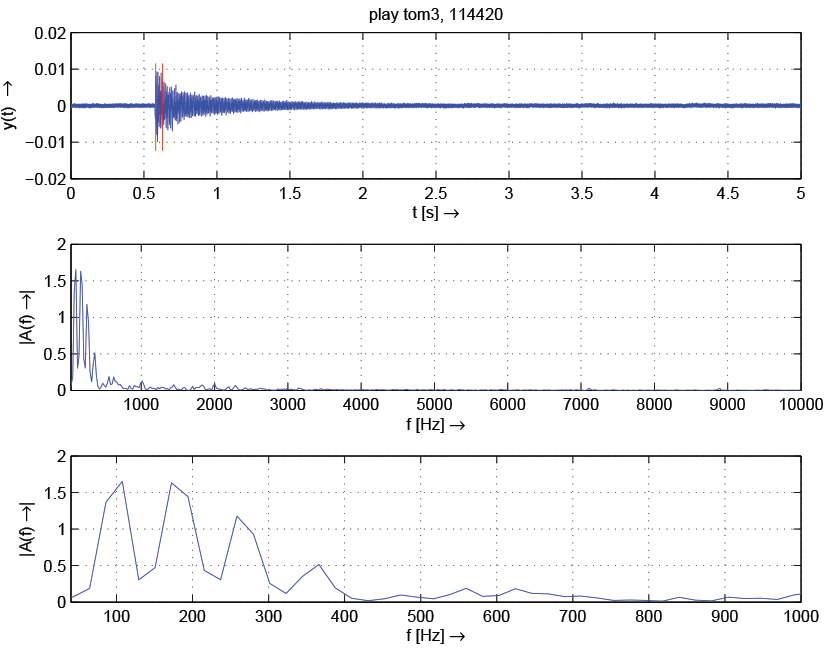
\includegraphics[height=5.5cm]{images/drum_spectra/play_tom3_114420_2048_0_plot_01_center.png}
		\label{fig:tom311}
	}
	\subfloat[Spectrogram]{
		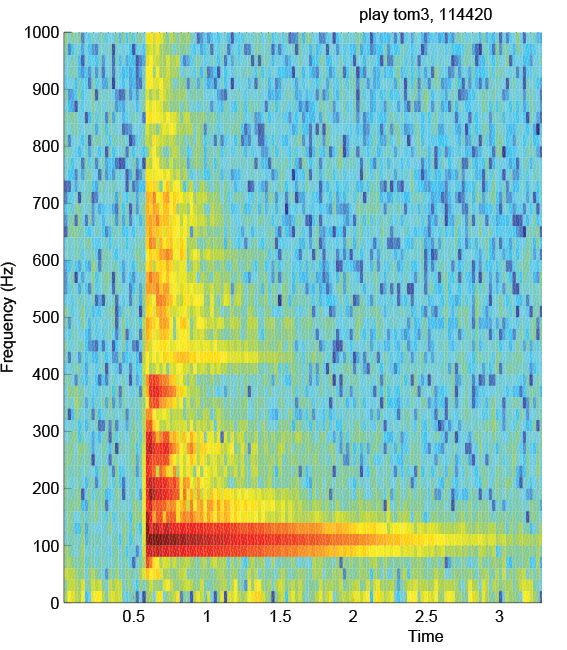
\includegraphics[height=5.5cm]{images/drum_spectra/play_tom3_114420_2048_0_plot_03_center.png}
		\label{fig:tom312}
	}
	\subfloat[Frames]{
		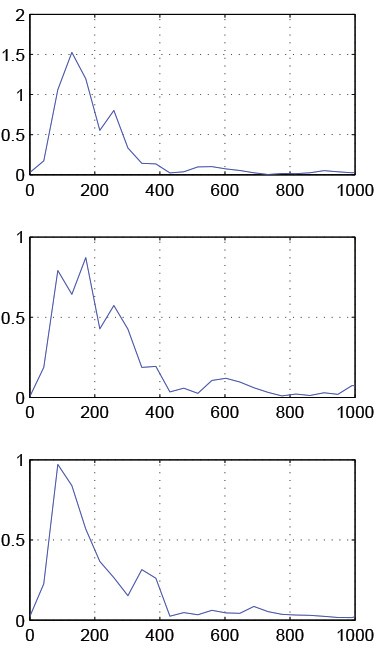
\includegraphics[height=5.5cm]{images/drum_spectra/play_tom3_114420_2048_0_plot_05_center.png}
		\label{fig:tom313}
	}
	\caption{Centered stroke with low power on tom 3}
	\label{fig:tom31}
\end{figure}

\begin{figure}
	\centering
	\subfloat[Time and Frequency domain]{
		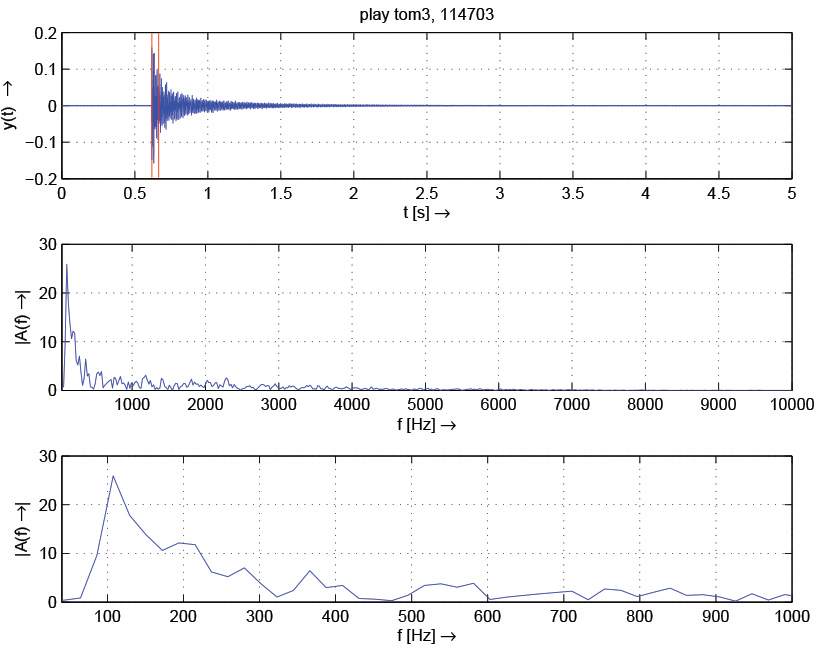
\includegraphics[height=5.5cm]{images/drum_spectra/play_tom3_114703_2048_0_plot_01_high.png}
		\label{fig:tom321}
	}
	\subfloat[Spectrogram]{
		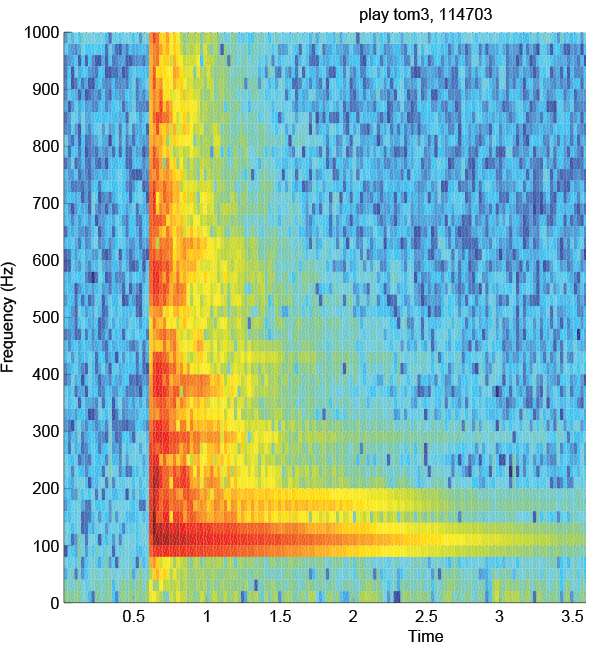
\includegraphics[height=5.5cm]{images/drum_spectra/play_tom3_114703_2048_0_plot_03_high.png}
		\label{fig:tom322}
	}
	\subfloat[Frames]{
		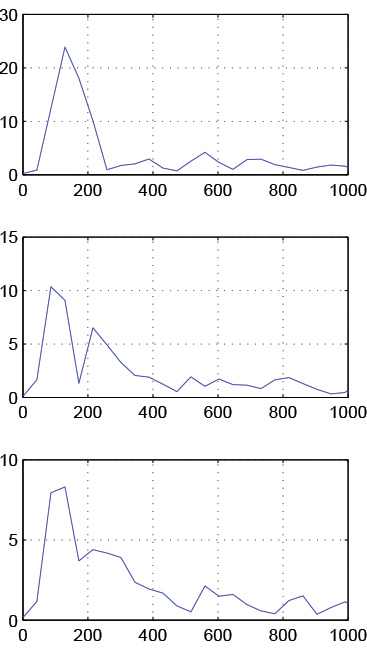
\includegraphics[height=5.5cm]{images/drum_spectra/play_tom3_114703_2048_0_plot_05_high.png}
		\label{fig:tom323}
	}
	\caption{Centered stroke with high power on tom 3}
	\label{fig:tom32}
\end{figure}

By examining the subsequent frames and spectrograms of all kinds of strokes on tom 3, it is considered that the frequency amplitudes and positions of the maximum peak are not stable over time, neither during the first 2048 samples nor over the entire duration of the stroke.

\begin{figure}
	\centering
	\subfloat[Time and Frequency domain]{
		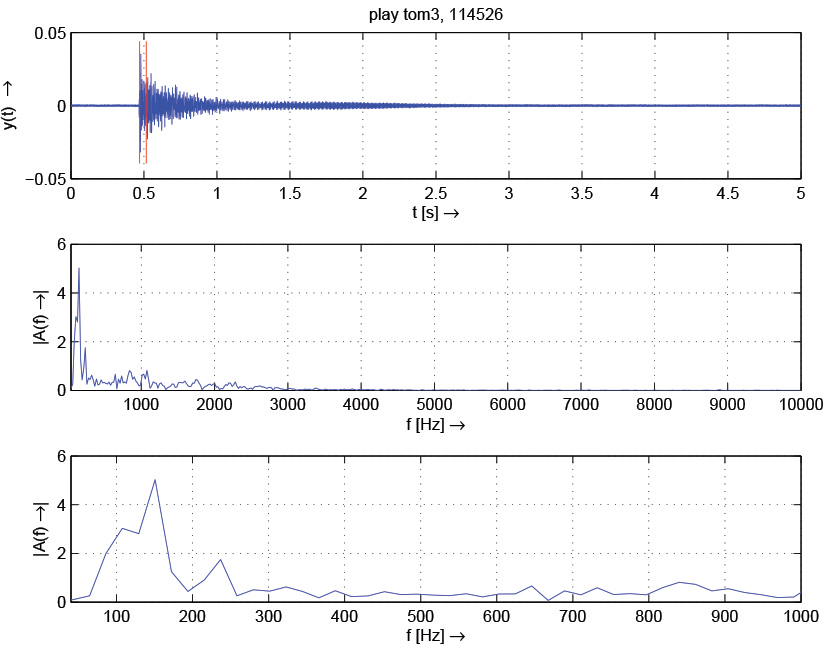
\includegraphics[height=5.5cm]{images/drum_spectra/play_tom3_114526_2048_0_plot_01_edge.png}
		\label{fig:tom331}
	}
	\subfloat[Spectrogram]{
		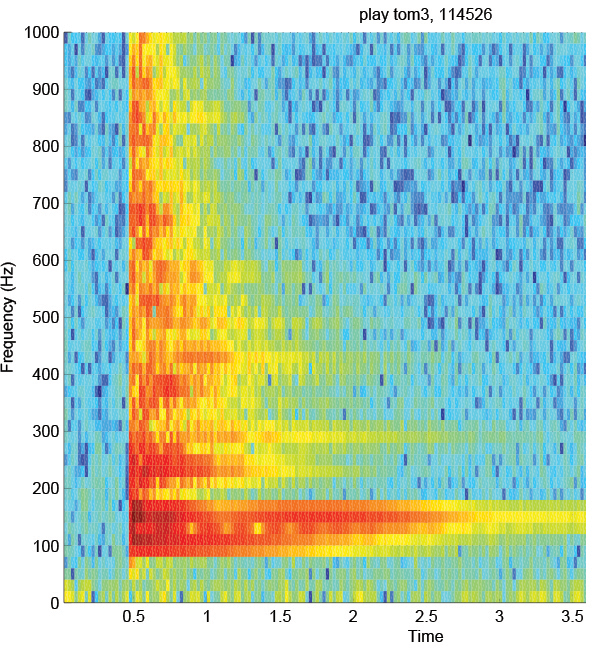
\includegraphics[height=5.5cm]{images/drum_spectra/play_tom3_114526_2048_0_plot_03_edge.png}
		\label{fig:tom332}
	}
	\subfloat[Frames]{
		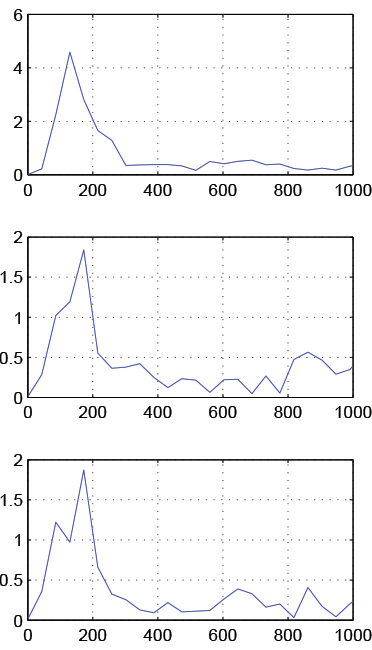
\includegraphics[height=5.5cm]{images/drum_spectra/play_tom3_114526_2048_0_plot_05_edge.png}
		\label{fig:tom333}
	}
	\caption{Stroke on the edge of tom 3}
	\label{fig:tom33}
\end{figure}


\subsubsection{Snare drum}

In contrast to other drum types, the snare has more frequency peaks, which also appear in a higher frequency range than 1000 Hz. This is caused by the rattles of gut on the backside head of the drum. These rattles produce more but lower, fast decaying peaks. So the most significant peaks, similar to the other drums, are located in a frequency band from 40 Hz to 1000 Hz. 

Very low or high powered strokes show an explicit peak at 194.6 Hz and several lower peaks. The lower peaks are varying for each stroke due to the sound produced by the rattles. Conspicuously, strokes with a medium power show a different spectral shape, which is less stable during the first few frames. This phenomena could also be produced by the rattles. It can appear if at this stroke intensity the sound of the rattles and the sound of the drum create similar frequency amplitude intensities. A medium stroke is displayed in figure \ref{fig:snare1}, a low and a high powered stroke in figure \ref{fig:snare2}.

\begin{figure}
	\centering
	\subfloat[Time and Frequency domain]{
		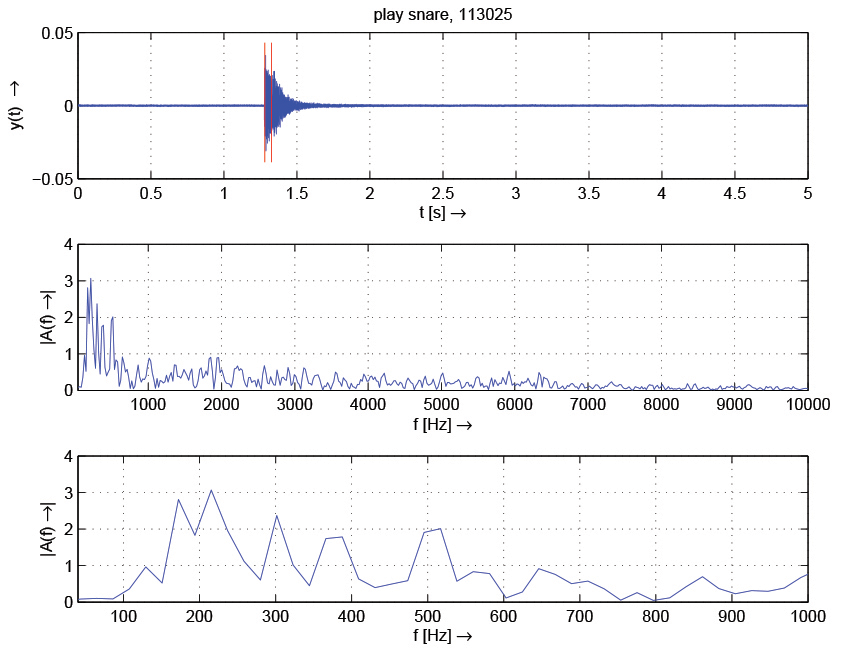
\includegraphics[height=5.5cm]{images/drum_spectra/play_snare_113025_2048_0_plot_01_center.png}
		\label{fig:snare12}
	}
	\subfloat[Spectrogram (0 - 10 kHz)]{  
		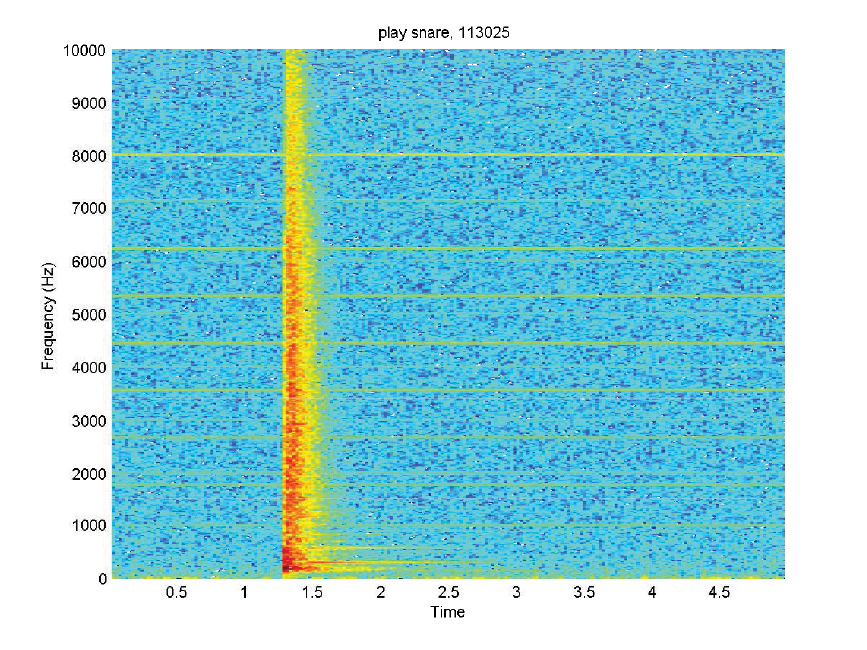
\includegraphics[height=5.5cm]{images/drum_spectra/play_snare_113025_2048_0_plot_02_center.png}
		\label{fig:snare12}
	}
	\qquad
	\subfloat[Time and Frequency domain]{
		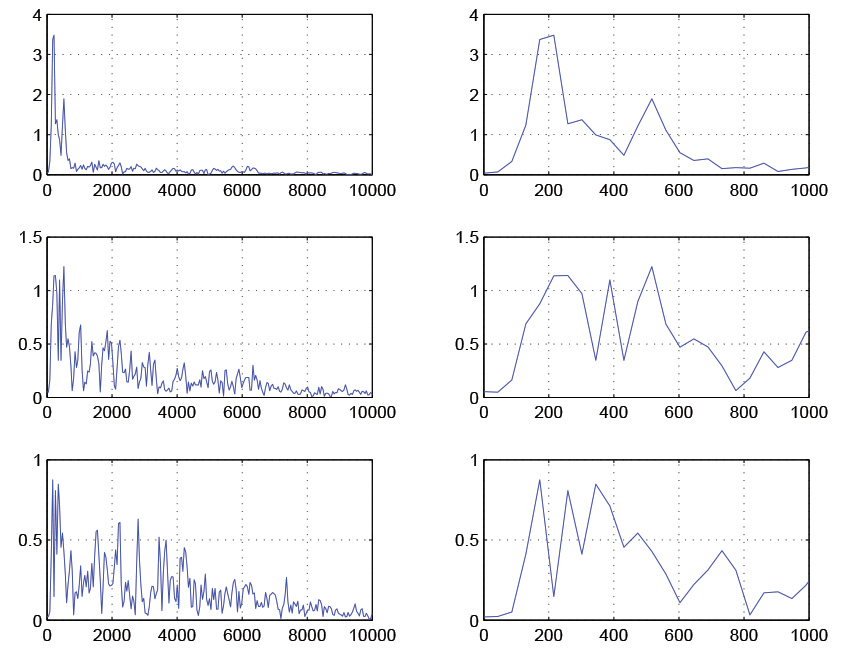
\includegraphics[height=5.5cm]{images/drum_spectra/play_snare_113025_2048_0_plot_05_center.png}
		\label{fig:snare11}
	}
	\subfloat[Spectrogram (0 - 1000 Hz)]{
		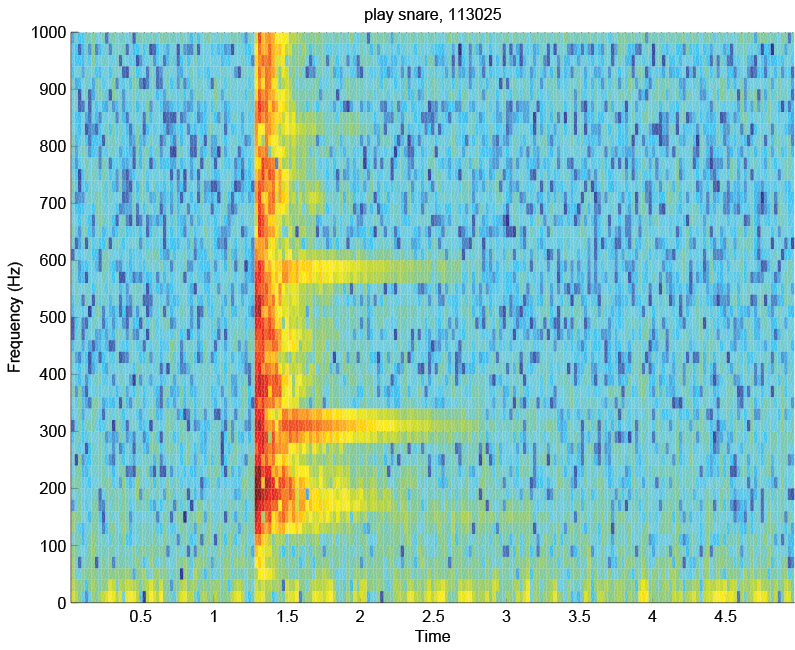
\includegraphics[height=5.5cm]{images/drum_spectra/play_snare_113025_2048_0_plot_03_center.png}
		\label{fig:snare13}
	}
	\caption{Centered stroke on the snare drum.}
	\label{fig:snare1}
\end{figure}


\begin{figure}
	\centering
	\subfloat[Low powered]{
		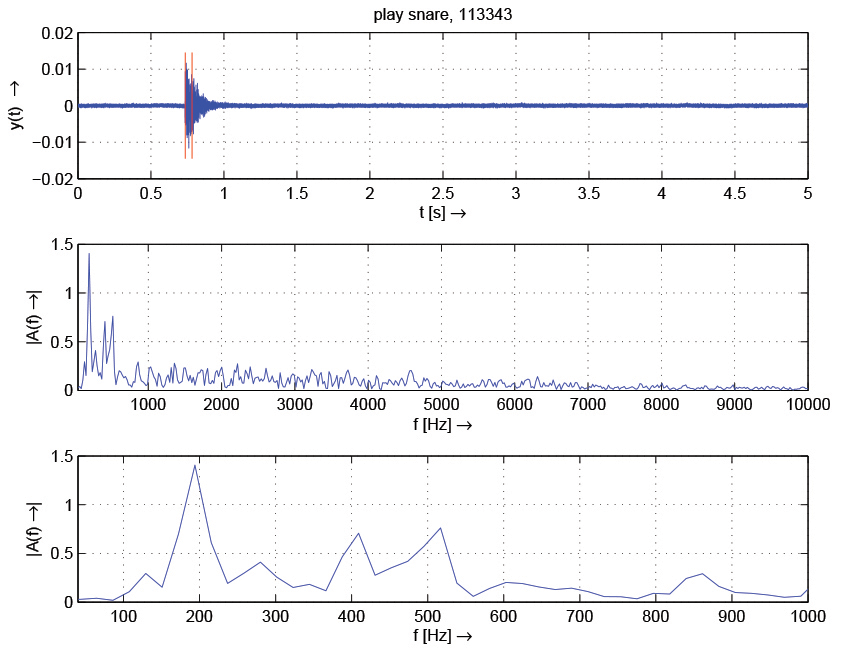
\includegraphics[width=7.3cm]{images/drum_spectra/play_snare_113343_2048_0_plot_01_low.png}
		\label{fig:snare21}
	}
	\subfloat[High powered]{
		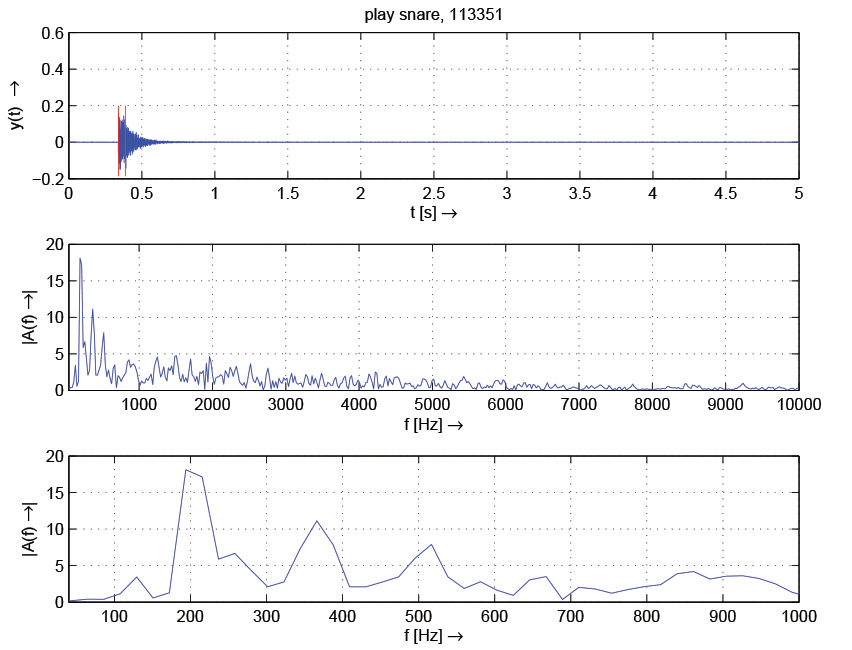
\includegraphics[width=7.3cm]{images/drum_spectra/play_snare_113351_2048_0_plot_01_high.png}
		\label{fig:snare22}
	}
	\caption{Different powered centered stroke on a snare drum.}
	\label{fig:snare2}
\end{figure}

As shown in figure \ref{fig:snare3}, additional frequency peaks appear for strokes at the edge of the drum head. 

\begin{figure}
	\centering
	\subfloat[Time and Frequency domain]{
		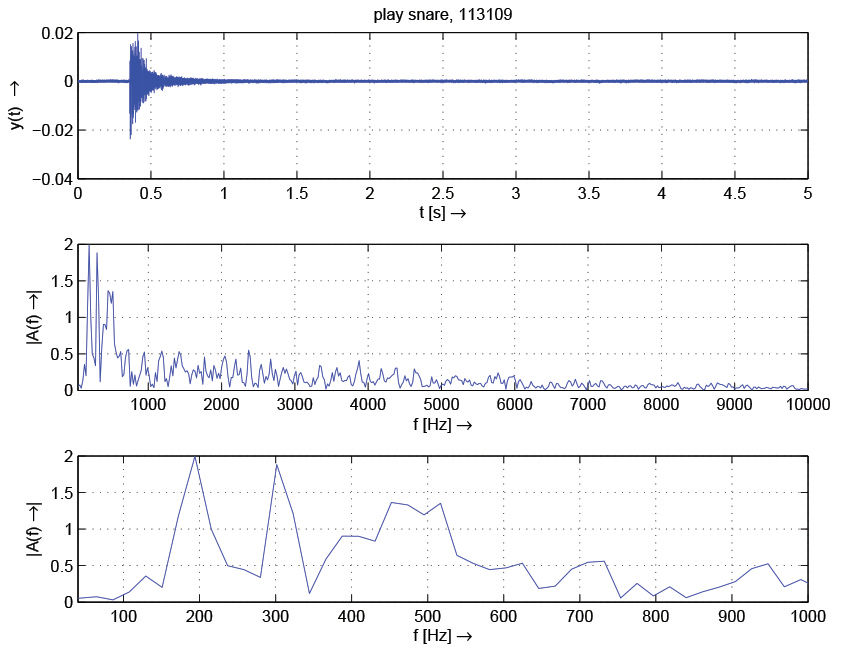
\includegraphics[height=5.5cm]{images/drum_spectra/play_snare_113109_2048_0_plot_01_edge.png}
		\label{fig:snare31}
	}
	\subfloat[Spectrogram (0 - 10 kHz)]{
		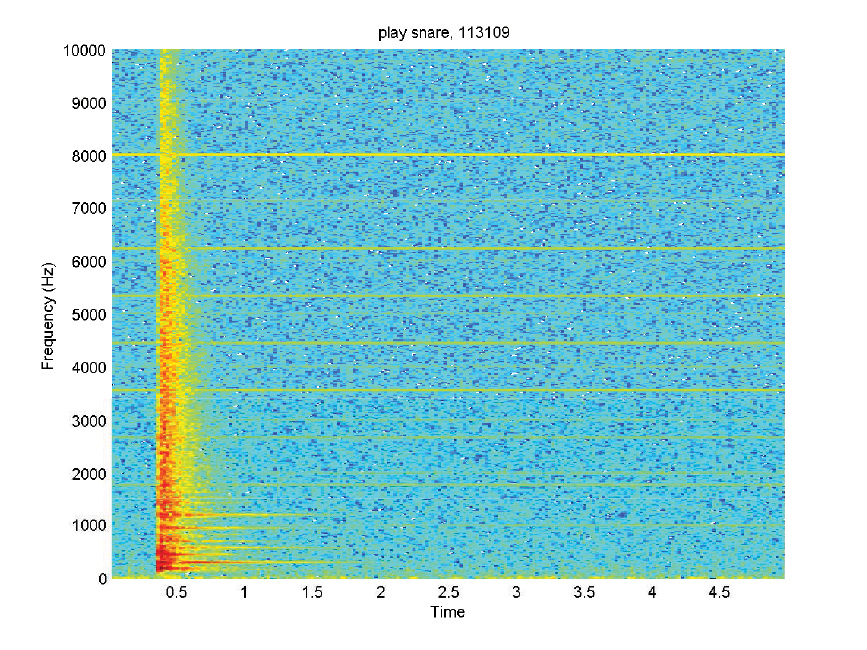
\includegraphics[height=5.5cm]{images/drum_spectra/play_snare_113109_2048_0_plot_02_edge.png}
		\label{fig:snare32}
	}
	\qquad
	\subfloat[Frames]{
		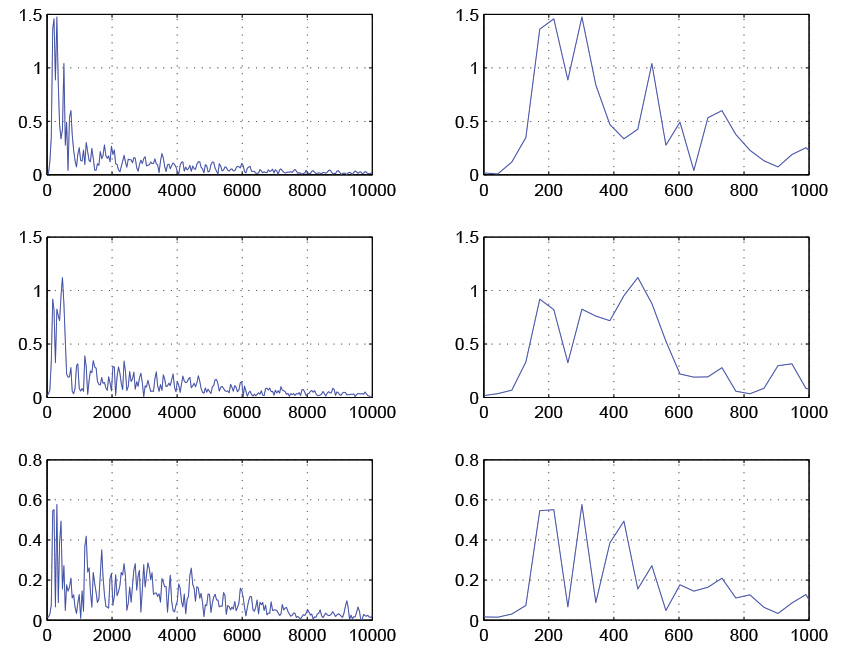
\includegraphics[height=5.5cm]{images/drum_spectra/play_snare_113109_2048_0_plot_05_edge.png}
		\label{fig:snare33}
	}
	\qquad
	\subfloat[Spectrogram (0 - 1000 Hz)]{
		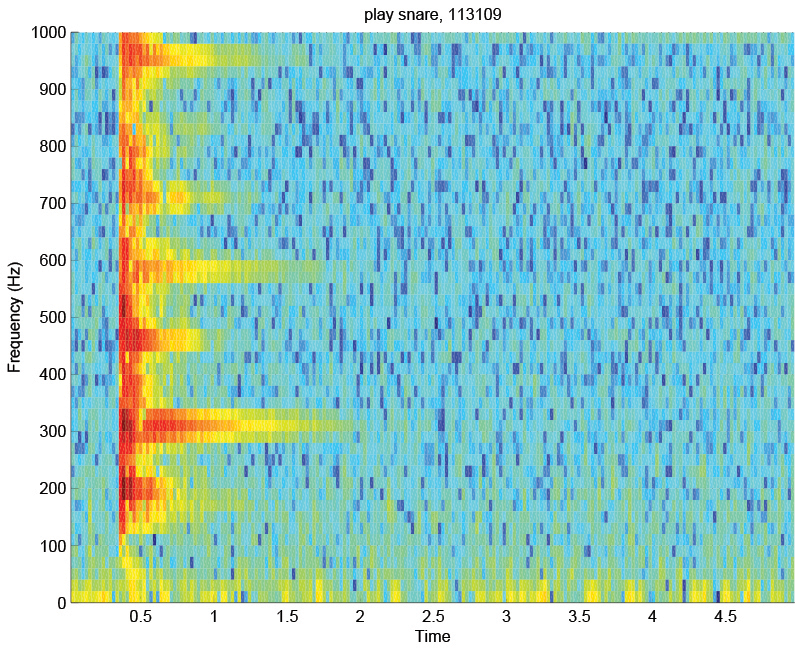
\includegraphics[height=5.5cm]{images/drum_spectra/play_snare_113109_2048_0_plot_03_edge.png}
		\label{fig:snare33}
	}
	\caption{Stroke at the edge of the snare drum.}
	\label{fig:snare3}
\end{figure}


\newpage
\subsubsection{Hi-hat}

The Hi-hat can be played opened or closed. Whereas the closed hi-hat produces a short bursting sound, the opened hi-hat's sound is clear and decays slowly. For this thesis, strokes on the rim of the hi-hat are considered for both opened and closed hi-hat's. In contrast to the drums, the hi-hat produces much more frequency peaks in a much broader spectrum, whereas the opened hi-hat produces less peaks than the closed one.

\begin{figure}[hbp]
	\centering
	\subfloat[Time and frequency domain stroke 1]{
		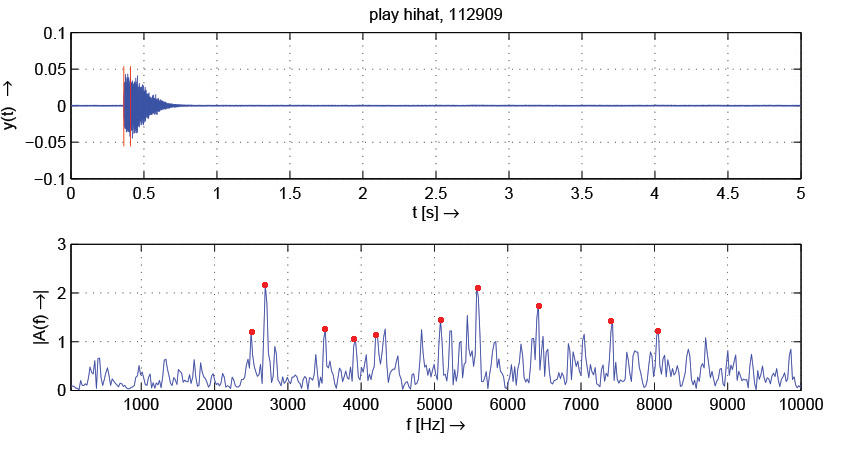
\includegraphics[width=7.2cm]{images/drum_spectra/play_hihat_112909_2048_0_plot_01_high2.png}
		\label{fig:hihat11}
	}
	\subfloat[Time and frequency domain stroke 2]{
		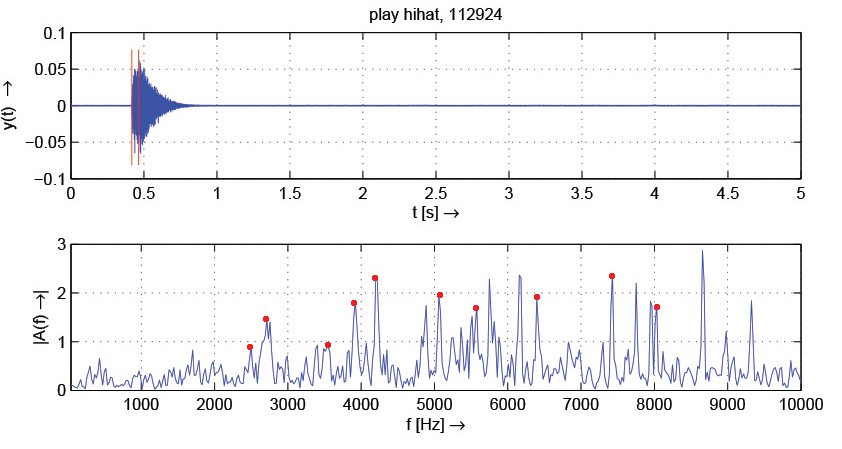
\includegraphics[width=7.2cm]{images/drum_spectra/play_hihat_112924_2048_0_plot_01_high2.png}
		\label{fig:hihat12}
	}
	\caption{Two equally powered strokes on the rim of a closed hi-hat.}
	\label{fig:hihat1}
\end{figure}

\begin{figure}[hbp]
	\centering
	\subfloat[Time and Frequency domain]{
		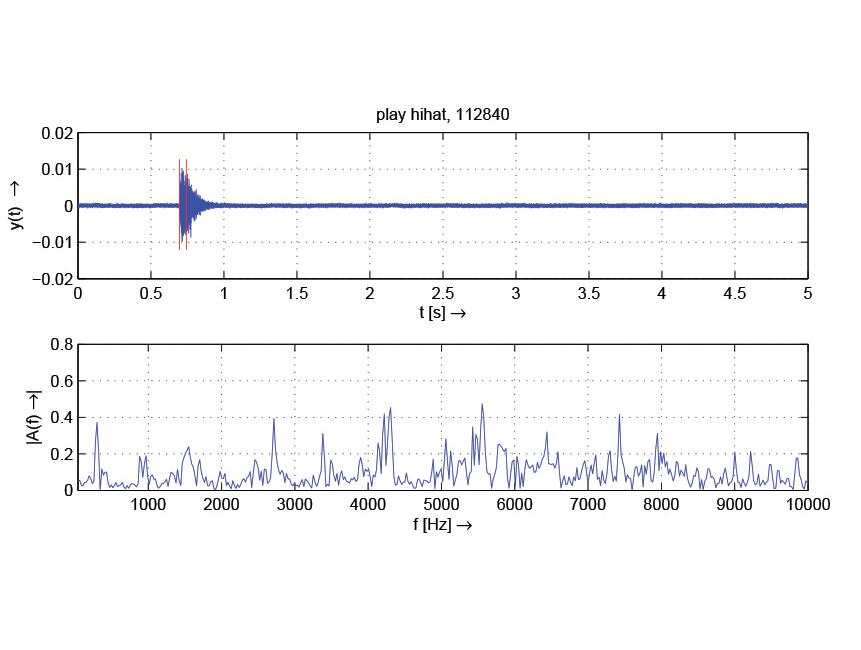
\includegraphics[height=5.5cm]{images/drum_spectra/play_hihat_112840_2048_0_plot_01_low.png}
		\label{fig:hihat21}
	}
	\subfloat[Spectrogram]{
		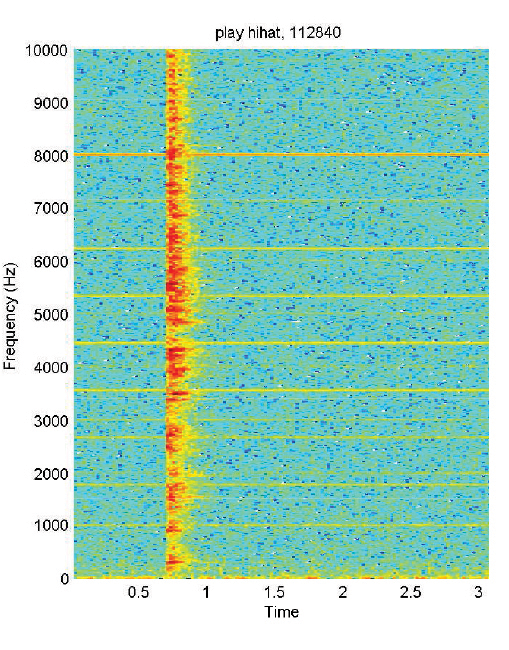
\includegraphics[height=5.5cm]{images/drum_spectra/play_hihat_112840_2048_0_plot_02_low.png}
		\label{fig:hihat22}
	}
	\subfloat[Frames]{
		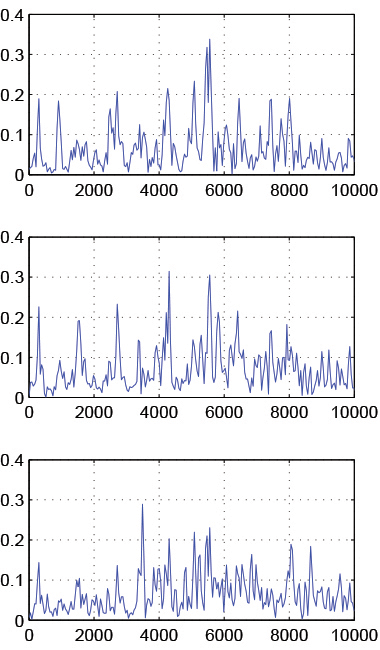
\includegraphics[height=5.5cm]{images/drum_spectra/play_hihat_112840_2048_0_plot_05_low.png}
		\label{fig:hihat23}
	}
	\caption{Low powered stroke on a closed hi-hat.}
	\label{fig:hihat2}
\end{figure}

%hihat closed
For strokes on a closed hi-hat the frequency spectra are varying from stroke to stroke. This is shown in figure \ref{fig:hihat1}. Here two equally powered strokes on the rim of the closed hi-hat are displayed. It is recognized that some peaks in the spectrum appear for both strokes, but with different intensities. The most significant of these peaks are marked red in the diagram. Further on, figure \ref{fig:hihat2} shows that also subsequent frames vary strongly.

As displayed in figure \ref{fig:hihat3}, for strokes with a higher power a clearer separation between low and high frequency peaks is observed. Furthermore, peaks appear in higher frequency ranges.

\begin{figure}
	\centering
	\subfloat[Time and Frequency domain]{
		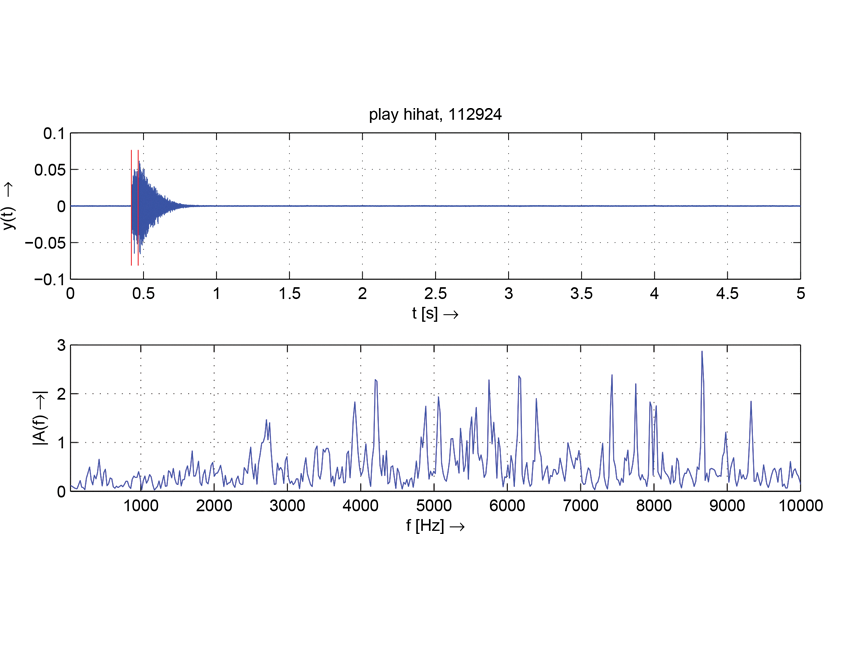
\includegraphics[height=5.5cm]{images/drum_spectra/play_hihat_112924_2048_0_plot_01_high.png}
		\label{fig:hihat31}
	}
	\subfloat[Spectrogram]{
		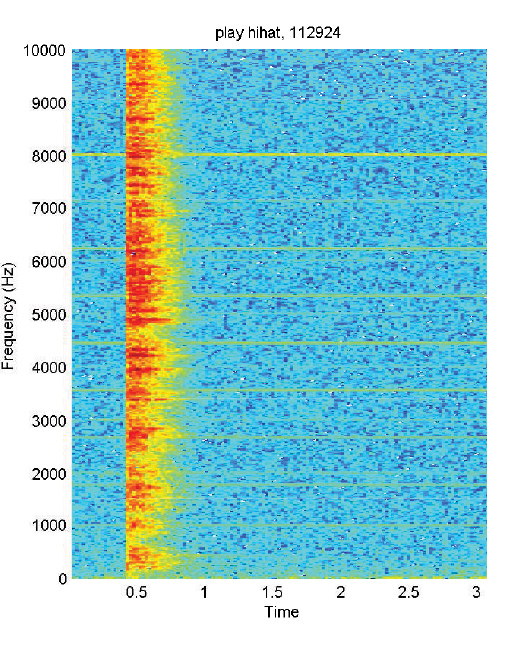
\includegraphics[height=5.5cm]{images/drum_spectra/play_hihat_112924_2048_0_plot_02_high.png}
		\label{fig:hihat32}
	}
	\subfloat[Frames]{
		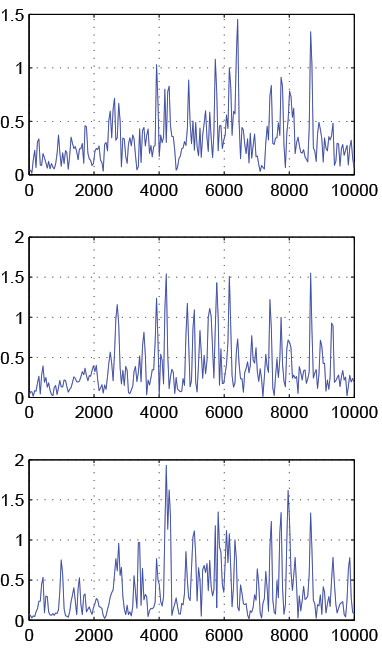
\includegraphics[height=5.5cm]{images/drum_spectra/play_hihat_112924_2048_0_plot_05_high.png}
		\label{fig:hihat33}
	}
	\caption{High powered stroke on a closed hi-hat.}
	\label{fig:hihat3}
\end{figure}

%hihat opened
For strokes on an opened hi-hat the peaks remain more stable if different strokes or subsequent frames are considered. More constant peaks appear between different strokes than for the closed hi-hat. For strokes with the same power the amplitudes stay more stable than for strokes with different powers. 

\begin{figure}
	\centering
	\subfloat[Time and frequency domain]{
		\includegraphics[height=3.4cm]{images/drum_spectra/play_hihat_open_112557_2048_0_plot_01_rim_low.png}
		\label{fig:hihat41}
	}
	\qquad
	\subfloat[Spectrogram]{
		\includegraphics[height=5.1cm]{images/drum_spectra/play_hihat_open_112557_2048_0_plot_02_rim_low.png}
		\label{fig:hihat42}
	}	
	\subfloat[Frames]{
		\includegraphics[height=5.1cm]{images/drum_spectra/play_hihat_open_112557_2048_0_plot_05_rim_low.png}
		\label{fig:hihat43}
	}
	\caption{Low powered stroke on an opened hi-hat.}
	\label{fig:hihat4}
\end{figure}

Moreover, for higher powered strokes, more frequency peaks in higher frequency ranges are observed than for low powered ones. When the sound decays, only a few of the peaks consist. These peaks remain the same during different strokes. Figure \ref{fig:hihat4} shows a low powered and figure \ref{fig:hihat5} a high powered stroke on the closed hi-hat.
	
\begin{figure}
	\centering
	\subfloat[Time and frequency domain]{
		\includegraphics[height=3.4cm]{images/drum_spectra/play_hihat_open_112641_2048_0_plot_01_rim_high.png}
		\label{fig:hihat51}
	}
	\qquad	
	\subfloat[Spectrogram]{
		\includegraphics[height=5.1cm]{images/drum_spectra/play_hihat_open_112641_2048_0_plot_02_rim_high.png}
		\label{fig:hihat52}
	}
	\subfloat[Frames]{
		\includegraphics[height=5.1cm]{images/drum_spectra/play_hihat_open_112641_2048_0_plot_05_rim_high.png}
		\label{fig:hihat53}
	}	
	\caption{High powered stroke on an opened hi-hat.}
	\label{fig:hihat5}
\end{figure}

\newpage
\subsubsection{Crash and Ride Cymbal}

The sound of the crash and ride cymbal is similar to the sound of the opened hi-hat. The crash cymbal creates a sharper, more crashing and higher frequent sound than the ride cymbal, which decays even slower with a shimmering sound. For the two cymbals, strokes on their rim, bow and bell are considered. The frequency spectra of the crash and ride cymbal also show similar properties to the hi-hat. Hence, figures \ref{fig:crash1} and \ref{fig:ride1} show that they produce frequency peaks persisting at equal frequency ranges with altering amplitudes. Thereby, they show less unstable peaks than the hi-hat. 

If the cymbals are stroked on the bow (figure \ref{fig:crashride1}), the peaks are more equally distributed over the frequency domain. Peaks also appear in higher frequency ranges than for cymbals stroked on their rim. The bell of a cymbal creates a much clearer sound than its rim or bow. The frequency spectra show less peaks than those for strokes on rim or bow. Especially, there are less peaks persisting over time. The distribution of the peak is equal to the distribution for strokes on the bow.

\begin{figure}[bp]
	\centering
	\subfloat[Time and frequency domain stroke 1]{
		\includegraphics[height=3.3cm]{images/drum_spectra/play_crash_snare_off_154836_2048_0_plot_01_rim.png}
		\label{fig:crash11}
	}
	\subfloat[Time and frequency domain stroke 2]{
		\includegraphics[height=3.3cm]{images/drum_spectra/play_crash_snare_off_154844_2048_0_plot_01_rim.png}
		\label{fig:crash12}
	}	
	\qquad
	\subfloat[Spectrogram stroke 1]{
		\includegraphics[height=5cm]{images/drum_spectra/play_crash_snare_off_154836_2048_0_plot_02_rim.png}
		\label{fig:crash13}
	}
	\subfloat[Spectrogram stroke 2]{
		\includegraphics[height=5cm]{images/drum_spectra/play_crash_snare_off_154844_2048_0_plot_02_rim.png}
		\label{fig:crash14}
	}		
	\caption{Equally powered strokes on the rim of the crash cymbal.}
	\label{fig:crash1}
\end{figure}

For different powered strokes, the crash and the ride cymbal show opposed properties, which can be seen in figure \ref{fig:crashride2}. For the crash cymbal, the emphasis of frequency peaks is in a frequency band between 0 Hz and 100 Hz for low powered strokes and in a frequency band from 2000 Hz to 5000 Hz for high powered strokes. Contrarily, for the ride cymbal, low powered strokes produce more frequency peaks in higher ranges (around 1000 Hz to 3000 Hz), whereas for high powered strokes, an explicit outstanding peak at 280 Hz is observed. Figure \ref{fig:ride22} shows that this peak stays consistent during the first 2048 samples.

Figure \ref{fig:crashride2} displays the subsequent frames. By comparing both figures it is figured out that the peaks for the crash cymbal are much more stable between the frames. The strokes on the bell create the most stable peaks for both cymbals. Furthermore, strokes on the bow are more stable than strokes on the rim and high powered strokes show more stable peaks than low powered ones.

\begin{figure}
	\centering
	\subfloat[Time and frequency domain stroke 1]{
		\includegraphics[height=3.3cm]{images/drum_spectra/play_ride_snare_off_154317_2048_0_plot_01_rim.png}
		\label{fig:ride11}
	}
	\subfloat[Time and frequency domain stroke 2]{
		\includegraphics[height=3.3cm]{images/drum_spectra/play_ride_snare_off_154325_2048_0_plot_01_rim.png}
		\label{fig:ride12}
	}	
	\qquad
	\subfloat[Spectrogram stroke 1]{
		\includegraphics[height=5cm]{images/drum_spectra/play_ride_snare_off_154317_2048_0_plot_02_rim.png}
		\label{fig:ride13}
	}
	\subfloat[Spectrogram stroke 2]{
		\includegraphics[height=5cm]{images/drum_spectra/play_ride_snare_off_154325_2048_0_plot_02_rim.png}
		\label{fig:ride14}
	}	
	\caption{Equally powered strokes on the rim of the ride cymbal.}
	\label{fig:ride1}
\end{figure}

\begin{figure}
	\centering
	\subfloat[Time and frequency domain crash]{
		\includegraphics[height=3.3cm]{images/drum_spectra/play_crash_snare_off_154855_2048_0_plot_01_bow.png}
		\label{fig:crashride11}
	}	
	\subfloat[Time and frequency domain ride]{
		\includegraphics[height=3.3cm]{images/drum_spectra/play_ride_snare_off_154409_2048_0_plot_01_bow.png}
		\label{fig:crashride12}
	}
	\qquad
	\subfloat[Spectrogram crash]{
		\includegraphics[height=5cm]{images/drum_spectra/play_crash_snare_off_154855_2048_0_plot_02_bow.png}
		\label{fig:crashride13}
	}	
	\subfloat[Spectrogram ride]{
		\includegraphics[height=5cm]{images/drum_spectra/play_ride_snare_off_154409_2048_0_plot_02_bow.png}
		\label{fig:crashride14}
	}	
	\caption{Strokes on the bow of the crash and the ride cymbal.}
	\label{fig:crashride1}
\end{figure}

\begin{figure}
	\centering
	\subfloat[Time and frequency domain crash]{
		\includegraphics[height=3.3cm]{images/drum_spectra/play_crash_snare_off_155005_2048_0_plot_01_bell.png}
		\label{fig:crashride11}
	}	
	\subfloat[Time and frequency domain ride]{
		\includegraphics[height=3.3cm]{images/drum_spectra/play_ride_snare_off_154528_2048_0_plot_01_bell.png}
		\label{fig:crashride12}
	}
	\qquad
	\subfloat[Spectrogram crash]{
		\includegraphics[height=5cm]{images/drum_spectra/play_crash_snare_off_155005_2048_0_plot_02_bell.png}
		\label{fig:crashride13}
	}	
	\subfloat[Spectrogram ride]{
		\includegraphics[height=5cm]{images/drum_spectra/play_ride_snare_off_154528_2048_0_plot_02_bell.png}
		\label{fig:crashride14}
	}	
	\caption{Strokes on the bell of the crash and the ride cymbal.}
	\label{fig:crashride1}
\end{figure}

\begin{figure}
	\centering
	\subfloat[crash low]{
		\includegraphics[height=3.3cm]{images/drum_spectra/play_crash_snare_off_155045_2048_0_plot_01_low.png}
		\label{fig:crashride21}
	}	
	\subfloat[ride low]{
		\includegraphics[height=3.3cm]{images/drum_spectra/play_ride_snare_off_154557_2048_0_plot_01_low.png}
		\label{fig:crashride22}
	}	
	\qquad
	\subfloat[crash high]{
		\includegraphics[height=3.3cm]{images/drum_spectra/play_crash_snare_off_155140_2048_0_plot_01_high.png}
		\label{fig:crashride23}
	}	
	\subfloat[ride high]{
		\includegraphics[height=3.3cm]{images/drum_spectra/play_ride_snare_off_154713_2048_0_plot_01_high.png}
		\label{fig:crashride24}
	}	
	\caption{Time and frequency domains of low and high powered strokes on crash and ride cymbal.}
	\label{fig:crashride2}
\end{figure}

\begin{figure}
	\centering	
	\subfloat[Crash rim low]{
		\includegraphics[height=5cm]{images/drum_spectra/play_crash_snare_off_154836_2048_0_plot_05_rim.png}
		\label{fig:crash21}
	}
	\subfloat[Crash rim high]{
		\includegraphics[height=5cm]{images/drum_spectra/play_crash_snare_off_155140_2048_0_plot_05_high.png}
		\label{fig:crash22}
	}
	\subfloat[Crash bow]{
		\includegraphics[height=5cm]{images/drum_spectra/play_crash_snare_off_154855_2048_0_plot_05_bow.png}
		\label{fig:crash23}
	}
	\subfloat[Crash bell]{
		\includegraphics[height=5cm]{images/drum_spectra/play_crash_snare_off_155005_2048_0_plot_05_bell.png}
		\label{fig:crash24}
	}
	\qquad	
	\subfloat[Ride rim low]{
		\includegraphics[height=5cm]{images/drum_spectra/play_ride_snare_off_154557_2048_0_plot_05_low.png}
		\label{fig:ride21}
	}		
	\subfloat[Ride rim high]{
		\includegraphics[height=5cm]{images/drum_spectra/play_ride_snare_off_154713_2048_0_plot_05_high.png}
		\label{fig:ride22}
	}
	\subfloat[Ride bow]{
		\includegraphics[height=5cm]{images/drum_spectra/play_ride_snare_off_154409_2048_0_plot_05_bow.png}
		\label{fig:ride23}
	}		
	\subfloat[Ride bell]{
		\includegraphics[height=5cm]{images/drum_spectra/play_ride_snare_off_154528_2048_0_plot_05_bell.png}
		\label{fig:ride24}
	}	
	\caption{Subsequent frames for different strokes on the crash and ride cymbal.}
	\label{fig:crashride2}
\end{figure}

